\documentclass[11pt]{article}
%Gummi|065|=)
\title{\textbf{Algorithms in Julia}}
\author{Valentin Churavy \and James Schloss}
\date{}

\usepackage{graphicx}
\usepackage{hyperref}
\usepackage{listings}
\usepackage{color}

\definecolor{dkgreen}{rgb}{0,0.6,0}
\definecolor{gray}{rgb}{0.5,0.5,0.5}
\definecolor{mauve}{rgb}{0.58,0,0.82}

\lstset{frame=tb,
  language=python,
  aboveskip=3mm,
  belowskip=3mm,
  showstringspaces=false,
  columns=flexible,
  basicstyle={\small\ttfamily},
  numbers=none,
  numberstyle=\tiny\color{gray},
  keywordstyle=\color{blue},
  commentstyle=\color{dkgreen},
  stringstyle=\color{mauve},
  breaklines=true,
  breakatwhitespace=true,
  tabsize=3
}


\begin{document}
\maketitle
In this document, we have descriptions of the following algorithms:
\begin{itemize}
\item Monte Carlo
\item Split-Operator method for solving the Schrodinger Equation
\item Julia Fractal
\item Force Integration with Verlet integration
\item Barnes-Hut (N-body galaxy simulation)
\item Euler Method
\item Subsetting Dataframes
\item Auto-Differentiation
\end{itemize}

All algorithms can be found in the examples directory of the \texttt{skillpill-julia} repository on github

\newpage
\section*{Monte Carlo}

There are many different methods that all work under the basic Monte Carlo principle of using random numbers to integrate systems.
For the sake of time and brevity, please refer to the following link for more information on Monte Carlo integration: \url{https://www.algorithm-archive.org/contents/monte_carlo_integration/monte_carlo_integration.html}. From there, modify the provided code to integrate $x^2$ where $-3 < x < 3$.

My function reads in a total range in x along with the number of points to sample. Try to match (or beat) the following benchmark:

\begin{lstlisting}
julia> @benchmark monte_carlo(6.0, 100000)
BenchmarkTools.Trial: 
  memory estimate:  0 bytes
  allocs estimate:  0
  --------------
  minimum time:     573.931 s (0.00% GC)
  median time:      578.105 s (0.00% GC)
  mean time:        596.870 s (0.00% GC)
  maximum time:     1.125 ms (0.00% GC)
  --------------
  samples:          8326
  evals/sample:     1

\end{lstlisting}


\newpage
\section*{Split-Operator Method}
The Split-Operator Method is a psuedo-spectral method that is important for many areas of physics, including quantum mechanics, where it is used to solve the Schr\"odinger equation,

$$
i \hbar \frac{\partial \Psi(\mathbf{r}, t)}{\partial t} = \left[\frac{-\hbar^2}{2m} \nabla^2 + V(\mathbf{r},t) \right] \Psi(\mathbf{r},t)
$$

To solve this equation, we basically split the time evolution operator ($\hat U = e^{-i \hat H t / \hbar}$) into 2 via the Baker-Campbell-Hausdorff relation:
$$\hat U_k = e^{-\mathbf{\hat p}^2 t / 2} \quad \hat U_V = e^{-V_0(\mathbf{\hat r})t/2}$$

From here, the method simply involves initializing the wavefunction and then multiplying it by half of $\hat U_V$ before flipping to momentum space via a FFT and multiplying it by all of $\hat U_k$ and then flipping back to real space with an inverse FFT and multiplying by the other half of $\hat U_V$, as shown in figure \ref{fig:split-op}.

More information can be found here: \url{https://www.algorithm-archive.org/contents/split-operator_method/split-operator_method.html}

\begin{figure}
\begin{center}
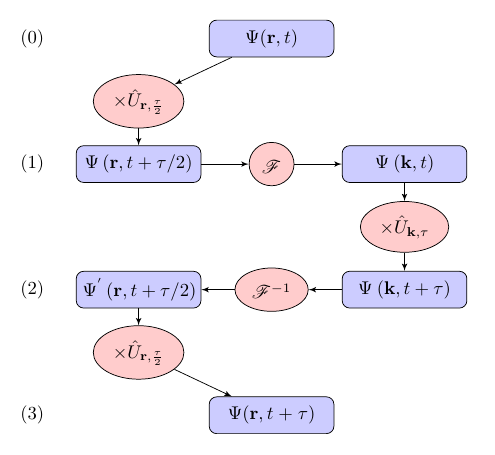
\includegraphics[width = 0.5\textwidth]{split-op.png}
\end{center}
\caption{A single step in the split-op method as described in the description}
\label{fig:split-op}
\end{figure}

\newpage
\section*{Julia Fractal}
Fractals are cool. They are structures that continually repeat themselves no matter how far you zoom in. Because we are using Julia, the obvious fractal to work with is the Julia fractal. Full implementation details in Python can be found here: \url{https://batchloaf.wordpress.com/2013/02/10/creating-julia-set-images-in-python/}. Basically, all we need to do is iteratively solve the following formula:
$$z_{n+1} = z_n^2 + c$$
Every iteration, we reduce pixel color by 5 and recalculate z until either the pixel color is 0 or $|z|$ exceeds a provided cutoff value (somewhat arbitrary). It should be noted here that $c$ is entirely complex and that the value dratically changes the output fractal.

Create the following: 
\begin{enumerate}
\item A function that sweeps through different $c$ values and outputs an image for each value
\item A function that zooms into a fractal of $c=1.0$ to see it's self-similar nature
\end{enumerate}

If you want to, you can even combine the images into a gif by using some additional tool (like ffmpeg)
\begin{figure}
\begin{center}
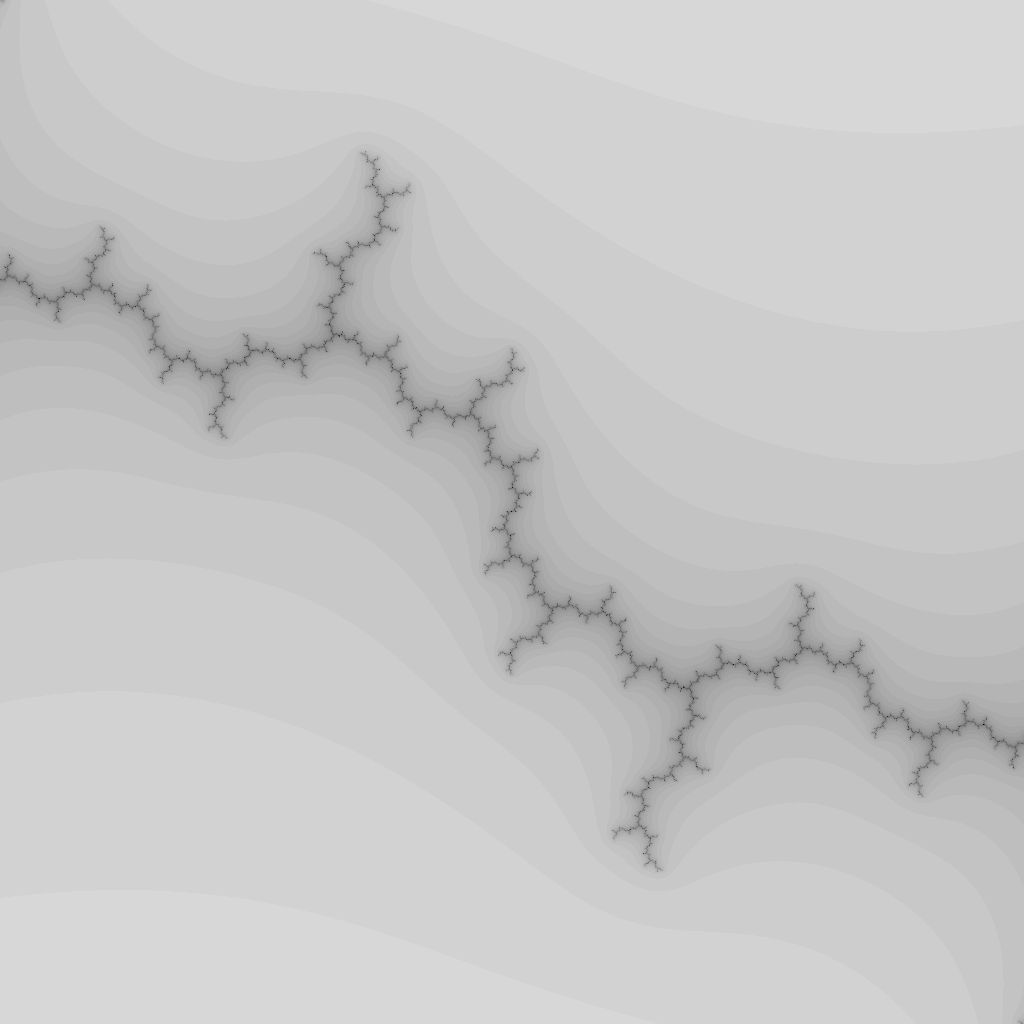
\includegraphics[width=0.45\textwidth]{fractal_zoom00030.png}
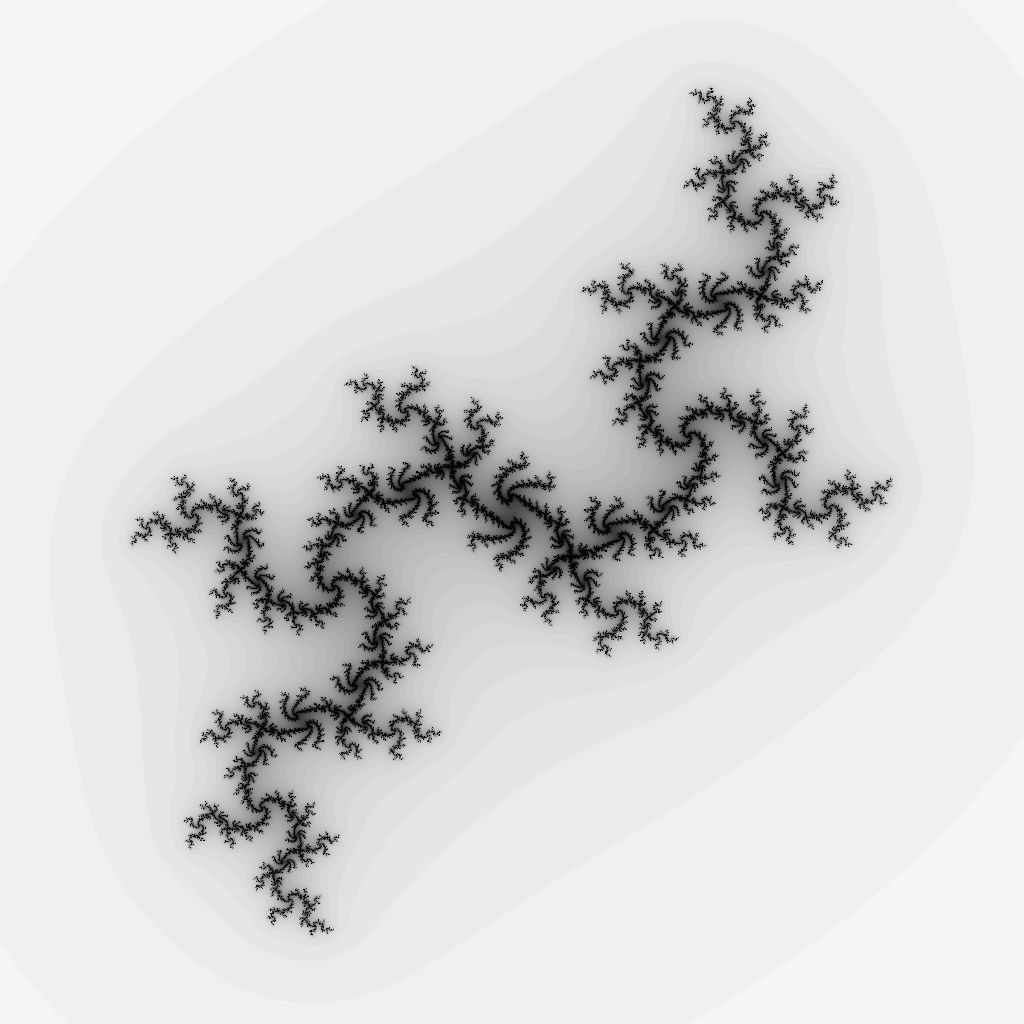
\includegraphics[width=0.45\textwidth]{c_scan00030.png}
\end{center}
\end{figure}

\newpage
\section*{Force Integration}
Integrating forces is a staple of any physics engine and most physics simulations. Though there are many different algorithms to do this, here we focus on the Verlet algorithm (because it's conceptually simple); however, if you want to implement Runge-Kutta (or whatever), feel free to do so!

First, let's start with the Taylor Series expansion:

$$x = x_0 + v_0 t + \frac{1}{2}at^2 + \ldots$$

If we are looking for $x(t + \Delta t)$, we can start by looking at the timesteps immediately before it:
$$x(t+\Delta t) = x(t) + v \cdot \Delta t + \frac{1}{2} a\cdot\Delta t^2$$
$$x(t-\Delta t) = x(t) - v \cdot \Delta t + \frac{1}{2} a\cdot\Delta t^2$$

Adding these together and solving for $x(t + \Delta t)$, we get:

$$x(t + \Delta t) = 2x(t) - x(t - \Delta t) + a \Delta t^2$$

This means we can solve for any object's new position if we know it's acceleration and where it's been! Of course, if we need the velocity (possibly to solve for the acceleration of a damped system), we can find it with:

$$v(t) = \frac{x(t + \Delta t) - x(t - \Delta t)}{2\Delta t}$$

Now, let's integrate some forces! Start with a ball at a height of 5m. How long does it take to hit the ground? Also, plot it's trajectory with time.

\newpage
\section*{Barnes-Hut}
Using the previous section on force integration, we know that all we really need for an N-body gravity simulator is a method to calculate the acceleration of an object in space. In principle, this is straightforward: We just add up all the particles and calculate

$$a = \frac{GMm}{r^2}$$

In practice, this means that we have an $O(n^2)$ problem on our hands! That said, we can take our N-body simulation and speed it up drastically with the help of a rather famous data structure known as an octree (or quadtree in 2d).

These data structures are straightforward. The root node is the entire simulation box, it's children are the octants of that box. Each octant has 8 octchildren, and we keep splitting up the simulation until every particle has it's own box. At this point, it's not obvious how this speed anything up; however, each box has a Center of Mass equal to all the elements on the inside of it. If our objects are sufficiently far away from each other, we can take a larger parent box instead of a smaller child box. This cuts computational time tremendously!

In particular, the cutoff value is defined as $\theta = s/d$ where $s$ is the width of the region represented by the internal node and $d$ is the distance between the body and it's Center of Mass. By playing with $\theta$, we can have either a fast, inaccurate simulation or a slow, accurate one. The trick is finding the happy-medium between the two!

\newpage
\section*{Euler Method}

Euler methods are some of the simplest methods for solving ordinary differential equations. For the purposes of this Skill Pill, we will only be implementing the forward Euler method, which is notably unstable with certain step sizes. Rather than doubling-up work that has already been done, please go to \url{https://www.algorithm-archive.org/contents/forward_euler_method/forward_euler_method.html}, and read up about the euler method there. There is even a Julia implementation available on the page if you are struggling to figure out how to do the implementation!

Admittedly, the primary author of the Algorithm Archive only solved a simple ODE: $y(t)' = -3t$; however, the method can easily be extended to other, more difficult equations!

\newpage
\section*{Subsetting Dataframes}

For many applications in computational science, it is important to learn how to appropriately use data frames. This was somewhat discussed earlier whith the \texttt{DelimitedFiles} and \texttt{CSV} packages; however, Julia should have all the features of other languages that are known for data frame manipulation, such as R.

To use a data frame, we first need to load the DataFrames package with \texttt{using DataFrames}. All of the documentation can be found here: \url{https://testdataframesjl.readthedocs.io/en/readthedocs/}. For this exercise, we will be a simple example of subsetting, which is a process of grabbing only a subset of the overall data frame. There is a lot more information about what is possible in the documentation, so feel free to mess around as you please!

In general, creating a data frame follows similar notation to creating arrays in Julia. If we wanted to create a matrix that has 3 columns (A, B, and C), all of which have different information, we might use the following command:

\begin{lstlisting}
df = DataFrame(A = 1:10, B = 2:2:20, C = (1:10).^2)
\end{lstlisting}

Which will create the following data frame:

\begin{lstlisting}
10x3 DataFrame
 Row  A      B      C     
      Int64  Int64  Int64 
 1    1      2      1     
 2    2      4      4     
 3    3      6      9     
 4    4      8      16    
 5    5      10     25    
 6    6      12     36    
 7    7      14     49    
 8    8      16     64    
 9    9      18     81    
 10   10     20     100   

\end{lstlisting}
Continued on next page...

\newpage
Here, we can grab particular elements by using the following operations:

\begin{lstlisting}
df[:B]   <- B column
df[1,2]  <- Row 1, column B
df[1:3] <- Rows 1-3
df[1:3, [:C,:A]] <- Columns C and A, rows 1-3
df[df[:A].%2 .== 0,:] <- all rows where A is even
\end{lstlisting}

so here is a quick problem set:

\begin{enumerate}
\item Create a data frame similar to the one created here
\item Use all the provided commands on the data frame
\item Turn all elements in column A to even by adding or subtracting 1 from all odd elements
\end{enumerate}

\newpage
\section*{Auto-differentiation}

I admittedly do not know much about auto-differentiation, but I plan to learn more. The purpose of this exercise is not to explain the theory of what auto-differentiation is or why it is important. Rather, this exercise intends to provide a succint description of auto-differentiation in Julia. For the most part, this is done with the \texttt{ForwardDiff.jl} package. The most up-to-date documentation can be found here: \url{http://www.juliadiff.org/ForwardDiff.jl/latest/index.html}.

The package provides Derivatives, Gradients, Hessians, and Jacobians, but for the purposes of this example, we will simply deal with derivatives.

Here is an example for doing a derivation of $f(x) = x^2$:

\begin{lstlisting}
f(x) = x^2
ForwardDiff.derivative(f,2)
\end{lstlisting}

This should output $4$ because $\frac{df(x)}{dx} = 2x$ and $2\times2 = 4$.

\vspace{1cm}

To get the hang of things from here, please compute the derivative of $\sin(x)$, evaluated at $x = 0$.

\vspace{1cm}

From there, please explore what you can do with the package and try to compute whatever derivatives you see fit!

\end{document}
